\documentclass{article}

\usepackage{coursenotes}

\usetikzlibrary{shapes,arrows}
\tikzset{%
pics/.cd,
nodea/.style args={#1#2#3}{
  code={\node[minimum height=2cm] (#3) {\color{#1}#2};
       \draw[thick] (#3.south west) -| (#3.north east)--(#3.north west);
  }
},
%pics/.cd,
nodeb/.style args={#1#2#3}{
  code={\node[minimum height=2cm] (#3) {\color{#1}#2};
       \draw[thick] (#3.south east) -| (#3.north west)--(#3.north east);
  }
},
%pics/.cd,
nodec/.style args={#1#2#3}{
  code={\node[draw,thick,shape=circle,inner sep=1cm] (#3) {\color{#1}#2};
  }
},
}

\set{AuthorName}{TC Fraser}
\set{Email}{tcfraser@tcfraser.com}
\set{Website}{www.tcfraser.com}
\set{ClassName}{Statistical Mechanics}
\set{School}{University of Waterloo}
\set{CourseCode}{Phys 359}
\set{InstructorName}{Michel Gingras}
\set{Term}{Winter 2016}

\begin{document}

\titlePage

\tableOfContents

\disclaimer

\section{Introduction}

\subsection{What is Statistical Mechanics}

Statistical Mechanics is thearea of Physics interested in systems with a large number of degress of freedon $n$. Note that these variables can be interacting or not. \\

There are two distinct class of Statistical Mechanics: equilibrium and non-equilibrium. \\

The Statistical part of Statistical Mechanics implies that it is inherently a study of probabilities and probability distributions. These laws must still remain fully consistent with physical laws. \\

Typically, systems are analyzed on a microscopic level. For a system of particles with charges $\bc{q_i}$ and their positions $\bc{\vr_i}$, the dynamics are governed by the forces acting on each particle,

\[ \vec{F}_i = m_i \vec{a}_i = \sum_{i\neq j} \f{q_iq_j}{4\pi\ep_0} \f{1}{\abs{\vec{r}_{ij}}^2} \]

But does labelling the particles really matter? For the case of $N \ar \infty$, the global phenomenology is of interest.

\subsection{History}

\begin{itemize}
    \item [1738] Daniel Bernoulli
    \begin{itemize}
        \item molecules moving in container, they collide with one another
        \item collisions with walls explains pressure
    \end{itemize}
    \item [$~$1850] Gay Lussac, Joule, Thomson (Lord Kelvin), Carnot
    \item [1859] James Clerk Maxwell
    \begin{itemize}
        \item $D(\nu) \sim e^{-\f{\nu^2}{2k_B T}}$
    \end{itemize}
    \item [1884] Josiash Willard Gibbs
    \begin{itemize}
        \item ensemble averaging
    \end{itemize}
    \item [$~$1900] Planck, Einstein, Bose, Pauli, Fermi, Dirac
    \item [Today] Frontier is in non-equilibrium Statistical Mechanics
    \begin{itemize}
        \item cold atoms
        \item biology
        \item quantum information
    \end{itemize}
\end{itemize}

\section{Foundations}

\subsection{Essence of Statistical Mechanics}

\heading{Laws of Thermodynamics}

\begin{tabular}{|c|c|}
    \hline
    Pros & Cons \\
    \hline
    \tabitem great because they are totally general &
    \tabitem does not tell us how to compute anything \\
    \tabitem relationship's (Maxwell's realtions) between $c_p, c_v, \al, \kappa$ &
    \tabitem does not tell us what entropy is \\
    \hline
\end{tabular} \\

The \nth{2} law of Thermodynamics reveals $\dif U = \indif Q - \indif W$ where $\indif Q = T \dif S$. \\

But what is $S$ and what does it \textbf{physically} mean? Boltzman reveals the relation:

\[ S = k_B \ln (\Om) \]

Which we will come back to.

\subsection{Postulate of Statistical Mechanics}

There is only one postulate of Statistical Mechanics:
\begin{displayquote}
    \textit{For an isolated system in equlibrium, all microstates accessible to the system are equally probable.}
\end{displayquote}

In order to digest this postulate, we will require some definitions.

\heading{Definitions}

\begin{itemize}
    \item system
    \begin{itemize}
        \item part of the universe we care about
        \item only weakly coupled to the rest of the universe
        \item the dynamics/mechanics are dominated by the internal degrees of freedom and forces
    \end{itemize}
    \item isolated
    \begin{itemize}
        \item idealization
        \item eliminates all external influences; no force, no energy/heat flux and no particle flux
        \item equantities such as the energy, number of particles and colume assumed constant forever $\dif U, \dif N, \dif V = 0$
    \end{itemize}
    \item equilibrium
    \begin{itemize}
        \item everything is no-longer changing
    \end{itemize}
    \item microstate
    \begin{itemize}
        \item a complete/total description of everything at the microscopic level $\bc{\vec{r}_i, \vec{p}_i}$ for each $i$
    \end{itemize}
    \item macrostate
    \begin{itemize}
        \item a decription at the macroscopic level in accordance with the external constraints
        \item $U, P, T, \bar{M}$
    \end{itemize}
    \item equally probable
    \begin{itemize}
        \item we are dealing with probabilities and statistics
        \item microstates are somehow describing probabilistically the properties at the macroscopic level
    \end{itemize}
    \item accessible
    \begin{itemize}
        \item  consistancy with the macroscopic constaints imposed by the conservation laws (fixed energy, fixed number of particles)
    \end{itemize}
\end{itemize}

\heading{Posulate Follow-up}

\begin{displayquote}
    \textit{We assume that the observed/realized macrostate is the one with the most microstates.}
\end{displayquote}

\subsection{Perspective from Coin Tossing}

Consider $4$ coins toassed many, many times. What are the microstates describing this system? \\

\newcolumntype{C}{>{\centering\arraybackslash}p{2em}}
\begin{tabular}{|c|CC|CCCC|c|c|}

\hline
Macrostate Label & \multicolumn{2}{c|}{Macrostate} & \multicolumn{4}{c|}{Microstate} & Thermo Probability & True Probability \\
{} & $N_H$ & $N_T$ & A & B & C & D & {} & {} \\
\hline
1 & 4 & 0 & H & H & H & H & 1 & $1/16$ \\
\hline
2 & 3 & 1 & H & H & H & T & 4 & $4/16$ \\
  &   &   & H & H & T & H &   & $    $ \\
  &   &   & H & T & H & H &   & $    $ \\
  &   &   & T & H & H & H &   & $    $ \\
\hline
3 & 2 & 2 & H & H & T & T & 6 & $6/16$ \\
  &   &   & H & T & T & H &   & $    $ \\
  &   &   & T & T & H & H &   & $    $ \\
  &   &   & T & H & H & T &   & $    $ \\
  &   &   & H & T & H & T &   & $    $ \\
  &   &   & T & H & T & H &   & $    $ \\
\hline
4 & 1 & 3 & T & T & T & H & 4 & $4/16$ \\
  &   &   & T & T & H & T &   & $    $ \\
  &   &   & T & H & T & T &   & $    $ \\
  &   &   & H & T & T & T &   & $    $ \\
\hline
5 & 0 & 4 & T & T & T & T & 1 & $1/16$ \\
\hline
\end{tabular}

\vspace{0.1in}

We note that the most probable macrostate $3$ is the one with the most microstates $6$. \\

How do we deal with very large $N, N_H, N_T$ in order to locate the most likely macrostate? First likes get a general expression for $\Om$ were $\Om$ is the number of microstates. Since $N = N_H + N_T$ and $N$ is considered fixed, there is only one free parameter $N_H$ (taken by choice). Thus $\Om$ can be considered a function of $N_H$ and nothing else. \\

Recall from probability that the form for $\Om$ is given by,

\[ \Om = \f{N!}{N_H!\br{N - N_H}!} \]

The most likely macrostate is given when $\Om$ (the number of microstates) is maximized. This means that we are interested in finding values of $N_H$, namely $N_H^*$ where,

\[ \bre{\der{\Om}{N_H}}_{N_H = N_H^*} = 0 \qquad \bre{\dder{\Om}{N_H}}_{N_H = N_H^*} > 0 \]

In order to do this, we will need to explore some mathematics ideas.

\subsection{Stirlings Formula and Gaussian Integrals}

Consider the integral,

\[ I = \intl_0^\inf x^N e^{-x} \dx \]

This can be evaluated using integration by parts,

\[ I = N \intl_0^\inf x^{N-1} e^{-x} \dx = \cdots = N! \numberthis \label{eq:intbypartsNtimes}\]

\subsubsection{Differentiation Trick}

However, integration by parts $N$ times on \eqref{eq:intbypartsNtimes} is annoying. There is a nice trick. Notice that,

\[ \intl_0^\inf e^{-ax} \dx = \bre{-\f1a e^{-ax}}_0^\inf = \f1a \numberthis \label{eq:tricka} \]

One can treat $a$ as a \textit{dummy} variable, and examine \eqref{eq:tricka}'s derivative with respect to $a$,

\[ \pder{}{a} \intl_0^\inf e^{-ax} \dx = \intl_0^\inf \pder{}{a} e^{-ax} \dx = \intl_0^\inf -x e^{-ax} \dx = \pder{}{a}\br{\f1a} = -\f{1}{a^2}\]

The reason for doing this is to simplify the process of \eqref{eq:intbypartsNtimes}. \\

If one explores the $N\tsp{th}$ derivative of \eqref{eq:tricka} with respect to $a$, you will derive the expression,

\[ \bs{\br{-1}^N \pderk{N}{}{a} \intl_0^\inf e^{-ax} \dx}_{a=1} = N! \numberthis \label{eq:trick} \]

The $\br{-1}^N$ term is a result of the alternating sign induced by bringing down a $-x$ each time you take a derivative. \\

\subsubsection{Stirling's Formula}

Looking back at the integral \eqref{eq:intbypartsNtimes},

\[ \intl_0^\inf x^N e^{-x} \dx = N! \numberthis \label{eq:stirlingstart}\]

How can we approximate $N!$ using the left had side of \eqref{eq:stirlingstart}? To derive Stirling's Formula, we need to make a change of variables $x = N + \sqrt{N} y$. Substituting into \eqref{eq:stirlingstart} gives,

\[ N! = \intl_0^\inf \sqrt{N} e^{-N} e^{N\ln\br{N+\sqrt{N}y}} e^{-\sqrt{N}y}\dy \]

The approimation begins by expanding the logarithm for large $N$,

\[ \ln\br{N + \sqrt{N}y} = \ln\br{N\bs{1+\f{y}{\sqrt{N}}}} = \ln\br{N} + \ln\br{1+\f{y}{\sqrt{N}}} \]

Take $\ep = \f{y}{\sqrt{N}} << 1$ and apply taylor series,

\[ \ln\br{1+\ep} \approx \ep - \f{\ep^2}{2} \]

Thus,

\[ N! \approx \sqrt{N}e^{-N}N^N\intl_{-\sqrt{N}}^\inf e^{-\f{y^2}{2}}\dy \]

The lower bound can be approximated as $\inf$ since $N$ is so large,

\[ N! \approx \sqrt{N}e^{-N}N^N\intl_{-\inf}^\inf e^{-\f{y^2}{2}}\dy \]

Notice the remaining integral term. It is called the \textit{Gaussian Integral} and has solution (see \nameref{sec:gaussianintegrals}),

\[ \intl_{-\inf}^\inf e^{-\f{y^2}{2}}\dy = \sqrt{\f{\pi}{a}} \numberthis \label{eq:gaussian} \]

Thus letting $a = 1/2$,

\[ N! \approx \sqrt{2\pi N}e^{-N}N^N \numberthis \label{eq:stirlinglong} \]

Equation \eqref{eq:stirlinglong} is known as \textit{Stirling's Formula}. However, there is a much more useful form of Stirling's Formula. It is obtained by taking the logarithm of both sides,

\[ \ln\br{N!} \approx \br{N+\f12}\ln\br{N} - \br{N - \untext{\f12 \ln\br{2\pi}}{small compared to large $N$}}  \]
\[ \ln\br{N!} \approx N\ln N - N \numberthis \label{eq:stirling} \]

Note that the remaining $N$ is not dropped. This is because for $N \sim 10^{23}$, $N\ln N - N$ and $N\ln N$ differ by about $2\%$. \\

Now we can apply this to the problem of maximizing $\Om$ (which is equivalent to mazimizing $\ln\Om$) because the logarithm is monotonically increasing.

\[ 0 = \pder{\ln\Om}{N_H} =\pder{}{N_H} \bs{\ln\br{\f{N!}{N_H!\br{N - N_H}!}}} \]

Through some manipulation, and applying \eqref{eq:stirling}, one obtains the expected result,

\[ N_H = \f{N}{2} \]

\subsubsection{Gaussian Integrals} \label{sec:gaussianintegrals}

Before continuing, we should take a moment to explore how \eqref{eq:gaussian} is solved. Let,

\[ I_x = \intl_{-\inf}^\inf e^{-ax^2}\dx \]

Here comes the trick. Multiply $I_x$ by itself and switch from rectangular coordinates to polar coordinates,

\[ I_xI_y = \intl_{-\inf}^\inf e^{-ax^2}\dx\intl_{-\inf}^\inf e^{-ay^2}\dy \]
\[ I^2 = \intl_{-\inf}^\inf\intl_{-\inf}^\inf e^{-a\br{x^2+y^2}}\dx\dy\]

Where we take $\R^2 (x, y) \mapsto \R^2 (r, \phi)$

\[ I^2 = \intl_{0}^{2\pi} \intl_{0}^\inf re^{-ar^2}\dif r\dif\phi\]

Which reveals that $I^2 = \pi/a$. Thus,

\[ I = \sqrt{\f{\pi}{a}} \]

\subsection{Connections between Thermodynamics and Statistical Mechanics}

Consider a lattice of $\text{Cu}^{2+}$ atoms. In a lattice the $\text{Cu}^{2+}$ atoms are distinguishable because they have unique locations. Now apply an external magnetic field.

\[ H\tsb{Zeeman} = - \vec{\mu} \cdot \vec{B} \]

Recall that $\vec{u} = g \mu_B \vec{s}$ has units $J/T$ where $T$ is tesla. Where for an electron,

\[ \mu_B = \f{e\hbar}{2m} = \SI{9e-24}{\joule \tesla^{-1}} \qquad g \approx 2 \]

For $\vec{B} = B \hat{z}$, $H\tsb{Zeeman} = 2\mu_BBs_z \defined b s_z$. The splitting of the two spin states $s_z = \pm 1$ for $B = \SI{1}{\tesla}$ has characteristic temperature of,

\[ \f{H\tsb{Zeeman}}{k_B} = \f{\vep}{k_B} = \f{\SI{10e-23}{\joule}}{\SI{1.4e23}{\joule\kelvin^{-1}}} \approx \SI{0.6}{\kelvin} \]

Now consider $N$ electrons subject to the field $\vec{B}$ where there are $N_+$ spins ``up'' and $N_-$ spins ``down''. This is completely analogous to the coin flipping example. The total energy of the system is given by,

\[ U = - N_- \vep + N_+ \vep \]

Note that $N = N_+ + N_-$ and thus,

\[ \f{U}{N} = \vep - 2 \vep \f{N_-}{N} \]

Constraining $U$ and using the substitution,

\[ \f{N_-}{N} = \f{1-x}{2} \qquad \f{N_+}{N} = \f{1+x}{2}\]

Then the microstate measure is given by,

\[ \Om = \f{N!}{N_+!N_-!} \]

Becomes (after some manipulation as using \eqref{eq:stirling})

\[ \ln\Om = -N\bs{\br{\f{1+x}{2}}\ln\br{\f{1+x}{2}} + \br{\f{1-x}{2}}\ln\br{\f{1-x}{2}}} \]

Now recall that for fixed volume $\dif V = 0$,

\[ \f{1}{T} = \br{\pder{S}{U}}_V \]

But since $U$ depends only on $x$, we can write,

\[ \f{1}{T} = \br{\pder{S}{x}}\br{\pder{x}{U}} \]

Thus reveals a slight connection between $S$ the entropy and $\Om$ through $x$ in this example. Further analysis with motivate Boltzman's equation,

\[ S = k_B \ln\Om + S_0 \]

\subsection{Example of a Physical System with Constraint}

Suppose you have $3$ partiables called $A,B,C$ such that each particle can have $\vep_j = j \vep$ where $j = 0, 1, 2, 3, \ldots$. \\

How many microstates are there subject to the constraint that the total energy is $3\vep$? \\

\begin{tabular}{|c|CCCC|CCC|c|c|}

\hline
Macrostate Label & \multicolumn{4}{c|}{Macrostate} & \multicolumn{3}{c|}{Microstate} & Thermo Probability & True Probability \\
{} & $N_0$ & $N_1$ & $N_2$ & $N_3$ & A & B & C & {} & {} \\
\hline
1 & 2 & 0 & 0 & 1 & 0 & 0 & $3\vep$ & 3 & $3/10$ \\
  &   &   &   &   & 0 & $3\vep$ & 0 &   &        \\
  &   &   &   &   & $3\vep$ & 0 & 0 &   &        \\
\hline
2 & 0 & 1 & 1 & 0 & 0 & $\vep$ & $2\vep$ & 6 & $6/10$ \\
  &   &   &   &   & $\vep$ & $2\vep$ & 0 &   &        \\
  &   &   &   &   & $2\vep$ & 0 & $\vep$ &   &        \\
  &   &   &   &   & 0 & $2\vep$ & $\vep$ &   &        \\
  &   &   &   &   & $2\vep$ & $\vep$ & 0 &   &        \\
  &   &   &   &   & $\vep$ & 0 & $2\vep$ &   &        \\
\hline
3 & 0 & 3 & 0 & 0 & $\vep$ & $\vep$ & $\vep$ & 1 & $1/10$ \\
\hline
\end{tabular}

\section{Review of Thermodynamics}

\subsection{Definitions}

Recall Boyle's Law $PV = nRT$.

\begin{itemize}
    \item processes
    \begin{itemize}
        \item constant $T$, isothermal process
        \item constant $P$, isobaric process
        \item constant $V$, isochoric process or isovolumetric process
        \item constant $S$, adiabatic process
        \begin{itemize}
            \item Comes from greek \textit{diabatos} which means \textit{to go through}
            \item No heat exchange between system and surroundings
            \item Can also be an approximation for processes that occur really quickly over a short period of time
        \end{itemize}
    \end{itemize}
    \item proceses reversible/irreversible
    \begin{itemize}
        \item reversible process happens over a number of dicrete steps and that are each reversibile
        \item irreversible processes are like poking a hole in a baloon or a gas expanding in a vacuum
    \end{itemize}
    \item thermodynamic variables $T, P, V, U$ where $U$ is the \textit{total energy}
\end{itemize}

\subsection{Zeroth Law of Thermodynamics}

If systems $A$ and $B$ are in equilibrium with one another and systems $B$ and $C$ are in equilibrium then $A$ is in equilibrium with $C$.

\subsection{Functions of State}

Thermodynamic varibales are not independent. They are often realted by an equation of state. For example $PV = nRT$ for an ideal gas. Other variables might come into an equation of state. For example $\rho, \mathcal{T}, E$ are all important for the equation of state for a liquid crystal sample. \\

Equations of state with typically look like

\[ f\br{P, V, T} = 0 \]

Another important notion is the notion of \textit{function of state}. A quantity that depends only on the thermodynamic variables of the system and \textit{not it's history}, is called a \textit{function of state}. \\

We will first focus on $U\tsb{total energy}$ first and then $S\tsb{entropy}$ as our functions of state. \\

Mathematically, $G = g\br{x,y}$ where $x,y$ are the thermodynamic variables and $G$ is a function of state analytic everywhere and obeys some properties:

\begin{itemize}
    \item $\dif G = \br{\pder{G}{x}}_y \dx + \br{\pder{G}{y}}_x \dy $
    \item at most values of the thermodynamic variables $g(x,y)$ is ``smooth''.
    \item for example: $\br{\pdder{G}{x}}_y$ or $\br{\pdder{G}{y}}_x$ or $\br{\pder{}{x}\br{\pder{G}{y}}_x}_y$ are all continous
    \item the order of discontinuities is determined by whether or not the system or substance is undergoing transitions of state or not
\end{itemize}

For functions of state that are analytical everywhere, the order of derivatives is inconsequential.

\[ \br{\pder{}{x}\br{\pder{G}{y}}} = \br{\pder{}{y}\br{\pder{G}{x}}}\]

What can we say about $G$ in cases where

\[ \dif G = \pder{G}{x} \dx + \pder{G}{y} \dy \numberthis \label{eq:dg} \]

in the case of functions of state like $U$, $ \dif U = \indif Q - \indif W  $ and the inexact differentials and how they relate to exact differentials like $\dif V$ and $\dif S$? In particular, when can we integrate $\dif U$?

Answer: eqaution \eqref{eq:dg} can be integrated in situations where

\[ \br{\pder{}{y}\br{\pder{G}{x}}_y}_x = \br{\pder{}{x}\br{\pder{G}{y}}_x}_y \numberthis \label{eq:exactcond}\]

When equation \eqref{eq:exactcond} is held for a physical system, one can say that $\dif G$ is an \textbf{exact differential}. Review 12,13 in notes on ``Review of Thermodynamics''. \\

The difference in the function $G(x,y)$ between two sufficiently close paris of points $(x_1, y_1)$ and $(x_2, y_2)$ depends only on the difference in $G(x,y)$ evaluated at those two points.

\[ \Delta G = G(x_2, y_2) - G(x_1, y_1) \]

$\Delta G$ does not depend on the path from point $(x_1, y_1)$ to $(x_1, y_1)$. In practice, one can assign such a function $G$ to the values of the thermodynamic variables at the points $(x,y)$. For example, $U(P,V)$ is such a function of state. It depends only on the description through the thermodynamic variables and not the history. \\

By counter example, heat $Q$ is not a function of state. No one can say, ``that substance has $X$ units of heat in it''.

\subsection{Work}

There are two types of work. One is called \textit{configuration work} and the other is called \textit{dissipative work}. \\

\subsubsection{Configuation Work}

Configuational work is denoted $\indif W$ where the symbol $\indif$ represents that it \textbf{is not} and exact differential.

\[ \indif W = \sum_i y_i \dif x_i \]

where $y_i$ is an intensive variable (not proportional to $N, V$; examples: pressure, surface tension). It can be thought of as a gneralized force. Here $\dif x_i$ is the generalized displacement which is an extensive variable.

\subsubsection{Dissipative Work}

Dissipative work can be thought of as ``stirring work''. Examples include a mixer in a liquid or an electrical wire/resistor.

\begin{itemize}
    \item electrical power:
    \begin{itemize}
        \item $P = V \cdot I$
        \item $\dif W\tsb{dis} = P \cdot \dif t = R I^2 \dif t$
    \end{itemize}
\end{itemize}

\subsubsection{Sign Convention}

\[ \indif W > 0 \note{work done by the system} \]
\[ \indif W < 0 \note{work done on the system} \]

Note:

\begin{itemize}
    \item work is \textbf{not} a property of the system
    \item work is \textbf{not} a function of state
    \item integration on a closed loop is not degenerate $\oint \indif W \neq 0$
\end{itemize}

\subsubsection{Abiabatic Work}

Abiabatic work occurs with no heat exchange.

\begin{center}
\begin{tikzpicture}[scale=1.0]
    % Draw axes
    \draw [<->,thick] (0,4) node (yaxis) [above] {$P$}
        |- (5,0) node (xaxis) [right] {$V$};
    \coordinate (f) at (4,1);
    \coordinate (i) at (1,3);
    \node [blue, label={[blue]10:$\indif Q = 0$}] (mid) at (2, 1.5) {};
    \draw [blue, thick, ->] plot [smooth, tension=1] coordinates { (i) (mid) (f)};
    \node [below] (vi) at (1,0) {$V_i$};
    \node [below] (vf) at (4,0) {$V_f$};
    \node [left] (pf) at (0,1) {$P_f$};
    \node [left] (pi) at (0,3) {$P_i$};
    \draw [gray, dashed] (i) -- (vi);
    \draw [gray, dashed] (i) -- (pi);
    \draw [gray, dashed] (f) -- (vf);
    \draw [gray, dashed] (f) -- (pf);
\end{tikzpicture}
\end{center}

Adiabatic work is done between any two equlibrium states and is \textit{independent of path}. One can define a function of state as the total adiabtic work done on a system. Lets define this a the total internal energy of the system.

\[ \dif U = - \dif W\tsb{adiabatic}\]

Note the minus `$-$' sign is due to the fact that the total energy of the system increases when work is done \textbf{on} this system. Along adiabatic paths, there is an exact differential associated with $\indif W$. It is called internal energy $\dif U$.

\subsection{First of Law of Thermodynamics}

\subsubsection{Heat}

In systems such as boiling a pot of water, there is no work performed on the system however the state of the system changes (not boiling to boiling). The mechanism that causes this change of state is heat ($Q$).

\[ \dif U = \indif W + \indif W \numberthis \label{eq:firstlaw} \]

Equation \eqref{eq:firstlaw} is using the following convention:

\begin{align*}
    \indif Q &:< 0 \note{heat flow \textbf{in}} \\
    \indif Q &:> 0 \note{heat flow \textbf{out}} \\
    \indif W &:< 0 \note{work is done \textbf{by} system} \\
    \indif W &:> 0 \note{work is done \textbf{on} system} \\
\end{align*}

\subsubsection{Heat Capacities}

Use the convention that $C$ is the heat capacity (extensive) and $c$ is the specific heat capacity (intensive).

\[ c = \f{C}{n} \]

\[ C \defined \lim_{\Delta T \ar 0} \f{\Delta Q}{\Delta T} \]

Heat capacity $C$ is very important. Measuring $C$ in a metal at low temperatures reveals very important intrinsic properties of the material. Also note that heat capacity is always $C \sim \f1T$ and not some other power than $-1$.

\heading{Relationship Between $c_v, c_p$ for an Ideal Gas}

\[ PV = nRT \]

Using Boyle's law, work with $n = \SI{1}{\mole}$ for convenience. How can we relate $C$ to the properties of the substance? Let us write (noting the `-' convention),

\[ \dif U = \indif Q - \indif W \]

Switch to specific (per mole) quantities,

\[ \dif u = \indif q - \indif w \]

\[ \dif u = \pdert{u}{T}{v} \dif T + \pdert{u}{v}{T} \dif V \]

\[ \indif q = \dif u + \indif w \]
\[ \indif q = \pdert{u}{T}{v} \dif T + \bc{\pdert{u}{v}{T} \dif V + P\dif v} \]

However,

\[ c_v = \lim_{\dif T \ar 0} \f{\indif q}{\dif T} \note{At constant V} \]

Thus,

\[ c_v = \pdert{u}{T}{v} \numberthis \label{eq:heatcapacity} \]

Which gives us,

\[ \indif q = c_v \dif T  + P\dif v \]

Note that this formula uses the fact that,

\[ \pdert{U}{v}{T} = 0 \note{For ideal gas.} \]

Which we will prove momentarily, but can be taken as an experimental fact discovered by Guy-Lussac. Namely $U$ is only a function of $T$ for an ideal gas ($U = U(T)$).

\[ \indif q = c_v \dif T  + P\dif v + \br{ v \dif p  - v\dif p} \]
\[ \indif q = \br{c_v + R} \dif T  - v\dif p \]

Thus,

\[ \lim_{\dif T \ar 0} \bre{\f{\indif q}{\dif T}}_{p=\text{const.}} = c_v + R \]

Thus we can define a new quantity,

\[ c_p \defined \bre{\f{\indif q}{\dif T}}_{p=\text{const.}} = c_v + R \]

For an monoatomic gas ($U = \f32 RT$),

\[ \ga \defined \f{c_p}{c_v} = \f{5}{3} \]

\subsection{Adiabatic Work Continued}

Let us examine an isotherm (red) next to an adiabatic curve (blue),

\begin{center}
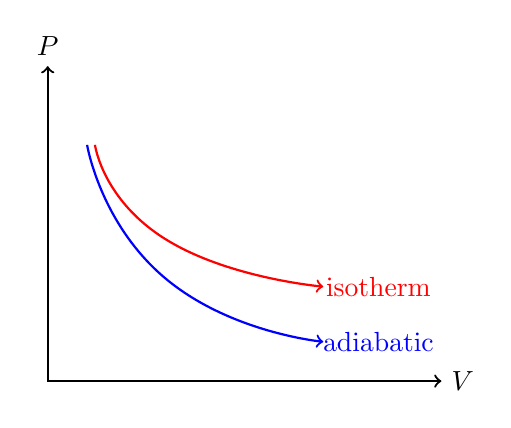
\begin{tikzpicture}[scale=1.0]
    % Draw axes
    \draw [<->,thick] (0,4) node (yaxis) [above] {$P$}
        |- (5,0) node (xaxis) [right] {$V$};
    \draw [blue, thick, ->] plot [smooth, tension=1] coordinates { (0.5,3) (1.5, 1.3) (3.5, 0.5)};
    \draw [red, thick, ->] plot [smooth, tension=1] coordinates { (0.6,3) (1.5, 1.8) (3.5, 1.2)};
    \node [blue] (adiabatic) at (4.2, 0.5) {adiabatic};
    \node [red] (isotherm) at (4.2, 1.2) {isotherm};
\end{tikzpicture}
\end{center}

\begin{align*}
    \indif q &= c_v \dif T + P \dif v \\
    \indif q &= c_P \dif T - v \dif P
\end{align*}

And let's set $\indif q = 0$ (adiabatic),

\[ c_v \dif T + P \dif v = c_P \dif T = v \dif P \]

Which gives,

\[ \f{\dif P}{P} = - \ga \f{\dif v}{v} \note{Using $\ga = c_P/c_v$} \]

Or integrating along a curve,

\[ \intl_1^2 \f{\dif P}{P} = - \intl_1^2 \ga \f{\dif v}{v} \]
\[ \ln\br{\f{P_2}{P_1}} = - \ga \ln\br{\f{v_2}{v_1}} \]

Which gives the relationship,

\[ P_1V_1^\ga = P_2V_2^\ga \]

Which holds true along an adiabatic curve. However, $PV = RT$. Thus using the expression $\dif U = - P \dif V |\tsb{adiabtic}$ gives the result,

\[ W = \bc{\f{P_2V_2 - P_1V_1}{1-\ga}}_{\ga > 1} \]

\subsubsection{Gay-Lussac Experiment}
\label{sec:guylussac}

For an ideal gas,

\[ \pdert{U}{V}{T} = 0 \]

\[ \indif Q = \pdert{U}{T}{V} \dif T + \bc{\pdert{U}{V}{T} + P}\dif V \]

\[ \f{\indif Q}{T} = \f{1}{T}\pdert{U}{T}{V} \dif T + \f{1}{T}\bc{\pdert{U}{V}{T} + P}\dif V \]

Employ an integrating factor for the inexact differentials. It will take us from and inexact differential to an exact differential.

\heading{Math Interlude}

\[ \indif G = A(x,y)\dx + B(x,y)\dy \]

Multiply $G$ by $\mu(x,y)$ and unknown function of $x$ and $y$,

\[ \dif \ti{G} = \mu \cdot \indif G\]

Thus,

\[ \dif \ti{G} = \mu A \dx + \mu B \dy \]

Making,

\[ \pder{\br{\mu A}}{y} = \pder{\br{\mu B}}{x} \numberthis \label{eq:intfact} \]

\heading{Example}

\[ \dif G = \sin(y) \dx + \cos(y) \dy \]
\[ \dif \ti{G} = \mu\sin(y) \dx + \mu\cos(y) \dy \]

Let us look for a $\mu$ such that $\mu(x,y) = \mu(x)$ and plugging into equation \eqref{eq:intfact},

\[ \pder{\br{\mu \sin(y)}}{y} = \pder{\br{\mu \cos(y)}}{x} \]
\[ \mu(x)\cos(y) = \der{\mu}{x}\cos(y) + \mu \der{\cos{y}}{x} \]
\[ \mu(x)\cancel{\cos(y)} = \der{\mu}{x}\cancel{\cos(y)} + \mu \cancelto{0}{\der{\cos{y}}{x}} \]

Thus,
\[ \mu(x) = \der{u}{x} \]
Which gives,
\[ \mu(x) = e^x \]

The purpose of introducing the notion of an integrating factor is to reveal that although $\indif Q$ is an inexact differential, we can introduce an integrating factor $\f1T$ that makes the quantity $\f{\indif Q}{T}$ an \textbf{exact} differential. This quantity is somehow more important that $Q$ as it describes a property of the system. We will see that this quantity is the motivation for entropy. Let us examine this,

\[ \f{\indif Q}{T} = \underbrace{\f{1}{T}\pdert{U}{T}{V}}_{A} \dif T + \underbrace{\f{1}{T}\bc{\pdert{U}{V}{T} + P}}_{B}\dif V \]

And thus,

\[ \pder{A}{V} = \pder{B}{T} \]

Gives,

\[ \pder{A}{V} = \pder{}{V}\bc{\f1T \pder{U}{T}} = \f1T \f{\partial^2 U}{\partial V \partial T} \]
\[ \pder{B}{T} = \pder{}{T}\bc{\f1T \br{\pder{U}{V} + P}} = -\f{1}{T^2} \br{\pder{U}{V} + P} + \f1T \f{\partial^2 U}{\partial T \partial V} + \f1T \pder{P}{T} \]

Equating these two expressions (noticing that $\f{\partial^2 U}{\partial T \partial V} = \f{\partial^2 U}{\partial V \partial T}$ and that $PV = RT \implies \f{P}{T^2} = \f{R}{TV}$),

\[ \f1T \f{\partial^2 U}{\partial V \partial T} = -\f{1}{T^2} \br{\pder{U}{V} + P} + \f1T \f{\partial^2 U}{\partial T \partial V} + \f1T \pder{P}{T} \]
\[ \cancel{\f1T \f{\partial^2 U}{\partial V \partial T}} = -\f{1}{T^2} \br{\pder{U}{V} + P} + \cancel{\f1T \f{\partial^2 U}{\partial T \partial V}} + \f1T \pder{P}{T} \]
\[ 0 = -\f{1}{T^2} \br{\pder{U}{V} + P} + \f1T \pder{P}{T} \]
\[ \f{1}{T^2} \br{\pder{U}{V} + P} = \f1T \pder{P}{T} \]
\[ \f{1}{T^2} \pder{U}{V} + \f{P}{T^2} = \f1T \pder{P}{T} \]
\[ \f{1}{T^2} \pder{U}{V} + \cancel{\f{R}{TV}} = \cancel{\f{R}{TV}} \]

Therefore Gay-Lussac was destined to find this realtionship through experiment:
\[ \pder{U}{V} = 0 \]

\subsubsection{Joule-Thomson(Kelvin) Experiment}

Using $\f{1}{T}$ as the integrating factor, one can go through a similar derivation as in section \ref{sec:guylussac} to understand that the quantity $S$ is a state function of a system with,

\[ \dif S \defined \f{\indif Q}{T}  \]

\subsubsection{Summary of First Law}

In summary, the first law of thermodynamics is really just conservation of energy with expression,

\[ \dif U = \indif Q - \indif W \]

\subsection{Second Law of Thermodynamics}

Physical laws on the microscopic scale always are found to have an inherent time-reversal symmetry. The physics behaves the same running forward in time and backward in time. However, a semi-paradox of real-world phenomenology seems to suggest that there are some processes can not occur moving backward in time. They still satisfy the conservation of energy, but there is another law that governs these macroscopic phenomena.

\subsubsection{Heat Engines}

Imagine a an engine $E$ that runs from temperature $T_2$ to $T_1$ (two heat baths), where it extracts heat $Q_2$ and disposes heat $Q_1$ and does some work $W$.

\begin{center}
\begin{tikzpicture}[scale=2]
    \pic at (0,0) {nodea={red}{$T_H$}{L}};
    \pic at (2,0) {nodec={black}{}{C}};
    \pic at (4,0) {nodeb={blue}{$T_C$}{R}};
    \draw[->,>=latex](L)--node[midway,above]{$Q_H$}(C);
    \draw[->,>=latex](C)--node[midway,above]{$Q_C$} (R);
    \draw[->,>=latex](C)--node[midway,left]{$W$} ++(0,-2cm);
\end{tikzpicture}
\end{center}

The efficiency of the engine is definied as,

\[ \eta \defined \f{\text{output}}{\text{input}} = \f{W}{Q_2} \]








\end{document}